\documentclass[t]{beamer}
\usefonttheme[onlymath]{serif}

\mode<presentation>
{
  \usetheme{Frankfurt}
  \usecolortheme{dove}  %% grey scale
  \useinnertheme{circles}
  % \setbeamercovered{transparent}
}

\hypersetup{
    colorlinks,
    citecolor=black,
    filecolor=black,
    linkcolor=black,
    urlcolor=blue
}
\usepackage{graphicx}

\graphicspath{ {../folding/sonobe-docs/src/imgs} }

\usepackage{listings} % embed code

\setbeamertemplate{itemize}{$\circ$}
\setbeamertemplate{itemize items}{$\circ$}

\beamertemplatenavigationsymbolsempty %% no navigation bar

\setbeamertemplate{footline}{\hspace*{.1cm}\scriptsize{
\hspace*{50pt} \hfill\insertframenumber/\inserttotalframenumber\hspace*{.1cm}\vspace*{.1cm}}}

\setbeamertemplate{caption}[numbered]
\setbeamerfont{caption}{size=\tiny}




\title{Anatomy of a folding scheme}
\author{\small{Sonobe, experimental folding schemes library implemented jointly by \href{https://0xparc.org}{0xPARC} and \href{https://pse.dev/}{PSE.}}}

\date{\vspace{1cm}\\\scriptsize{2024-04-22\\Barcelona zkDay}}

\begin{document}

\frame{\titlepage}


% To mention at the beginning:
% we would need more than 2h to show a bit of more detail, but we only have 20min


\section[Motivation]{Motivation}

\begin{frame}{Why folding}
  \begin{itemize}
    \item Repetitive computations take big circuits $\longrightarrow$ large proving time
    \begin{itemize}
      \item ie. prove a chain of 10k sha256 hashes
    \end{itemize}

    % \pause

    \item Traditional recursion: verify (in-circuit) a proof of the correct execution of the same circuit for the previous input
    \begin{itemize}
      \item issue: in-circuit proof verification is expensive (constraints)
      \begin{itemize}
        \item ie. verify a Groth16 proof inside a R1CS circuit
      \end{itemize}
    \end{itemize}
  \end{itemize}

  % draw: G16 proof being verified inside a circuit for which a new proof is generated
\end{frame}

\begin{frame}{IVC - Incremental Verifiable Computation}
  Folding schemes efficitently achieve IVC, where the prover recursively proves the correct execution of the incremental computations.

  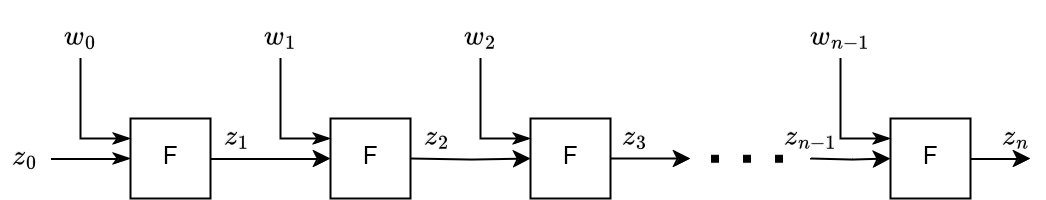
\includegraphics[width=\textwidth]{folding-main-idea-diagram}

  In other words, it allows to prove efficiently that $z_n = F(...~F(F(F(F(z_0, w_0), w_1), w_2), ...), w_{n-1})$.

\end{frame}


\begin{frame}{Folding idea}
  % draw of 2 instances being folded into a single one
  % then add other instances to show k-to-1 folding
\end{frame}


\section[Folding]{Folding}
\begin{frame}{Homomorphic commitments and RLC}
  We rely on homomorphic commitments\\
  ie. Pedersen commitments\\
  Let $g \in \mathbb{G}^n,~ v \in \mathbb{F}_r^n$,\\
  $$Com(v) = \langle g, v \rangle =g_1 \cdot v_1 + g_2 \cdot v_2 + \ldots + g_n \cdot v_n$$

  % \pause

  RLC:\\
  Let $v_1, v_2 \in \mathbb{F}_r^n$, set $cm_1 = Com(v_1),~ cm_2=Com(v_2)$.
  \\then,
  \begin{align*}
    v_3 &= v_1 + r \cdot v_2\\
    cm_3 &=cm_1 + r \cdot cm_2
  \end{align*}
  \\so that
  $$cm_3 = Com(v_3)$$

\end{frame}

\begin{frame}{Relaxed R1CS}
  R1CS instance: $(\{A, B, C\} \in \mathbb{F}^{n \times n},~ io,~ n,~ l)$, such that for $z=(io \in \mathbb{F}^l, 1, w \in \mathbb{F}^{n-l-1}) \in \mathbb{F}^n$,

$$Az \circ Bz = Cz$$

% \pause

Relaxed R1CS:

$$Az \circ Bz = uCz + E$$

for $u \in \mathbb{F},~~ E \in \mathbb{F}^n$.

\vspace{1cm}

Committed Relaxed R1CS instance: $CI = (\overline{E}, u, \overline{W}, x)$\\
Witness of the instance: $WI=(E, W)$

\vspace{0.5cm}
\footnotesize{(We don't have time for it now, but there is a simple reasoning for the RelaxedR1CS usage explained in Nova paper)}


\end{frame}

\begin{frame}{NIFS - Non Interactive Folding Scheme}
  \scriptsize{
  \begin{align*}
    CI_1 &=(\overline{E}_1 \in \mathbb{G}, u_1 \in \mathbb{F}, \overline{W}_1 \in \mathbb{G}, x_1 \in \mathbb{F}^n) ~~~~~~WI_1=(E_1 \in \mathbb{F}^n, W_1 \in \mathbb{F}^n)\\
    CI_2 &=(\overline{E}_2, u_2, \overline{W}_2, x_2) ~~~~~~WI_2=(E_2, W_2)
  \end{align*}
  where $\overline{V}=Com(V)$


% \pause

  \begin{align*}
    T &= Az_1 \circ Bz_1 + Az_2 \circ Bz_2 - u_1 C z_1 - u_2 C z_2\\
    \overline{T}&=Com(T)
  \end{align*}
  % \pause

\begin{minipage}[t]{.45\textwidth}
  NIFS.P
  \begin{align*}
    E &= E_1 + r \cdot T + r^2 \cdot E_2\\
    W &= W_1 + r \cdot W
  \end{align*}
\end{minipage}
\hfill\vline\hfill
\begin{minipage}[t]{.45\textwidth}
  NIFS.V
  \begin{align*}
    \overline{E} &= \overline{E}_1 + r \cdot \overline{T} + r^2 \cdot \overline{E}_2\\
    u &= u_1 + r \cdot u_2\\
    \overline{W} &= \overline{W}_1 + r \cdot \overline{W}\\
    x &= x_1 + r \cdot x_2
  \end{align*}
\end{minipage}

New folded Committed Instance: $(\overline{E}, u, \overline{W}, x)$\\
New folded witness: $(E, W)$
}
\end{frame}

\begin{frame}{IVC}
  \small{
  $U_i$: committed instance for the correct execution of invocations $1, \ldots, i-1$ of $F'$\\
  $u_i$: committed instance for the correct execution of invocation $i$ of $F'$
  }

  % draw: sketch of the Augmented F Circuit
  % big box for F', inside small box for F. NIFS.V box, how things connect to next iteration

  \vspace{4cm}
  
  \small{
  F':\\
  i) execute a step of the incremental computation, $z_{i+1} = F(z_i)$\\
  ii) invoke the NIFS.V to fold $U_i, u_i$ into $U_{i+1}$\\
  iii) other checks to ensure that the IVC is done properly
  }
\end{frame}

\begin{frame}{Cycle of curves}
  \small{
  NIFS.V involves $\mathbb{G}$ point scalar mults, which are not native over $\mathbb{F}_r$.
  \\$\longrightarrow$ delegate them into a circuit over a 2nd curve.

  \vspace{0.3cm}

  We 'mirror' the main $F'$ circuit into the 2nd curve\\
  each circuit computes natively the point operations of the other curve
  }

  % draw:
  % 1st the Nova with duplicated F' circuits over 2 curves
  % 2nd the Nova with CycleFold circuits sketch
\end{frame}


\begin{frame}{Augmented F Circuit + CycleFold Circuit}
  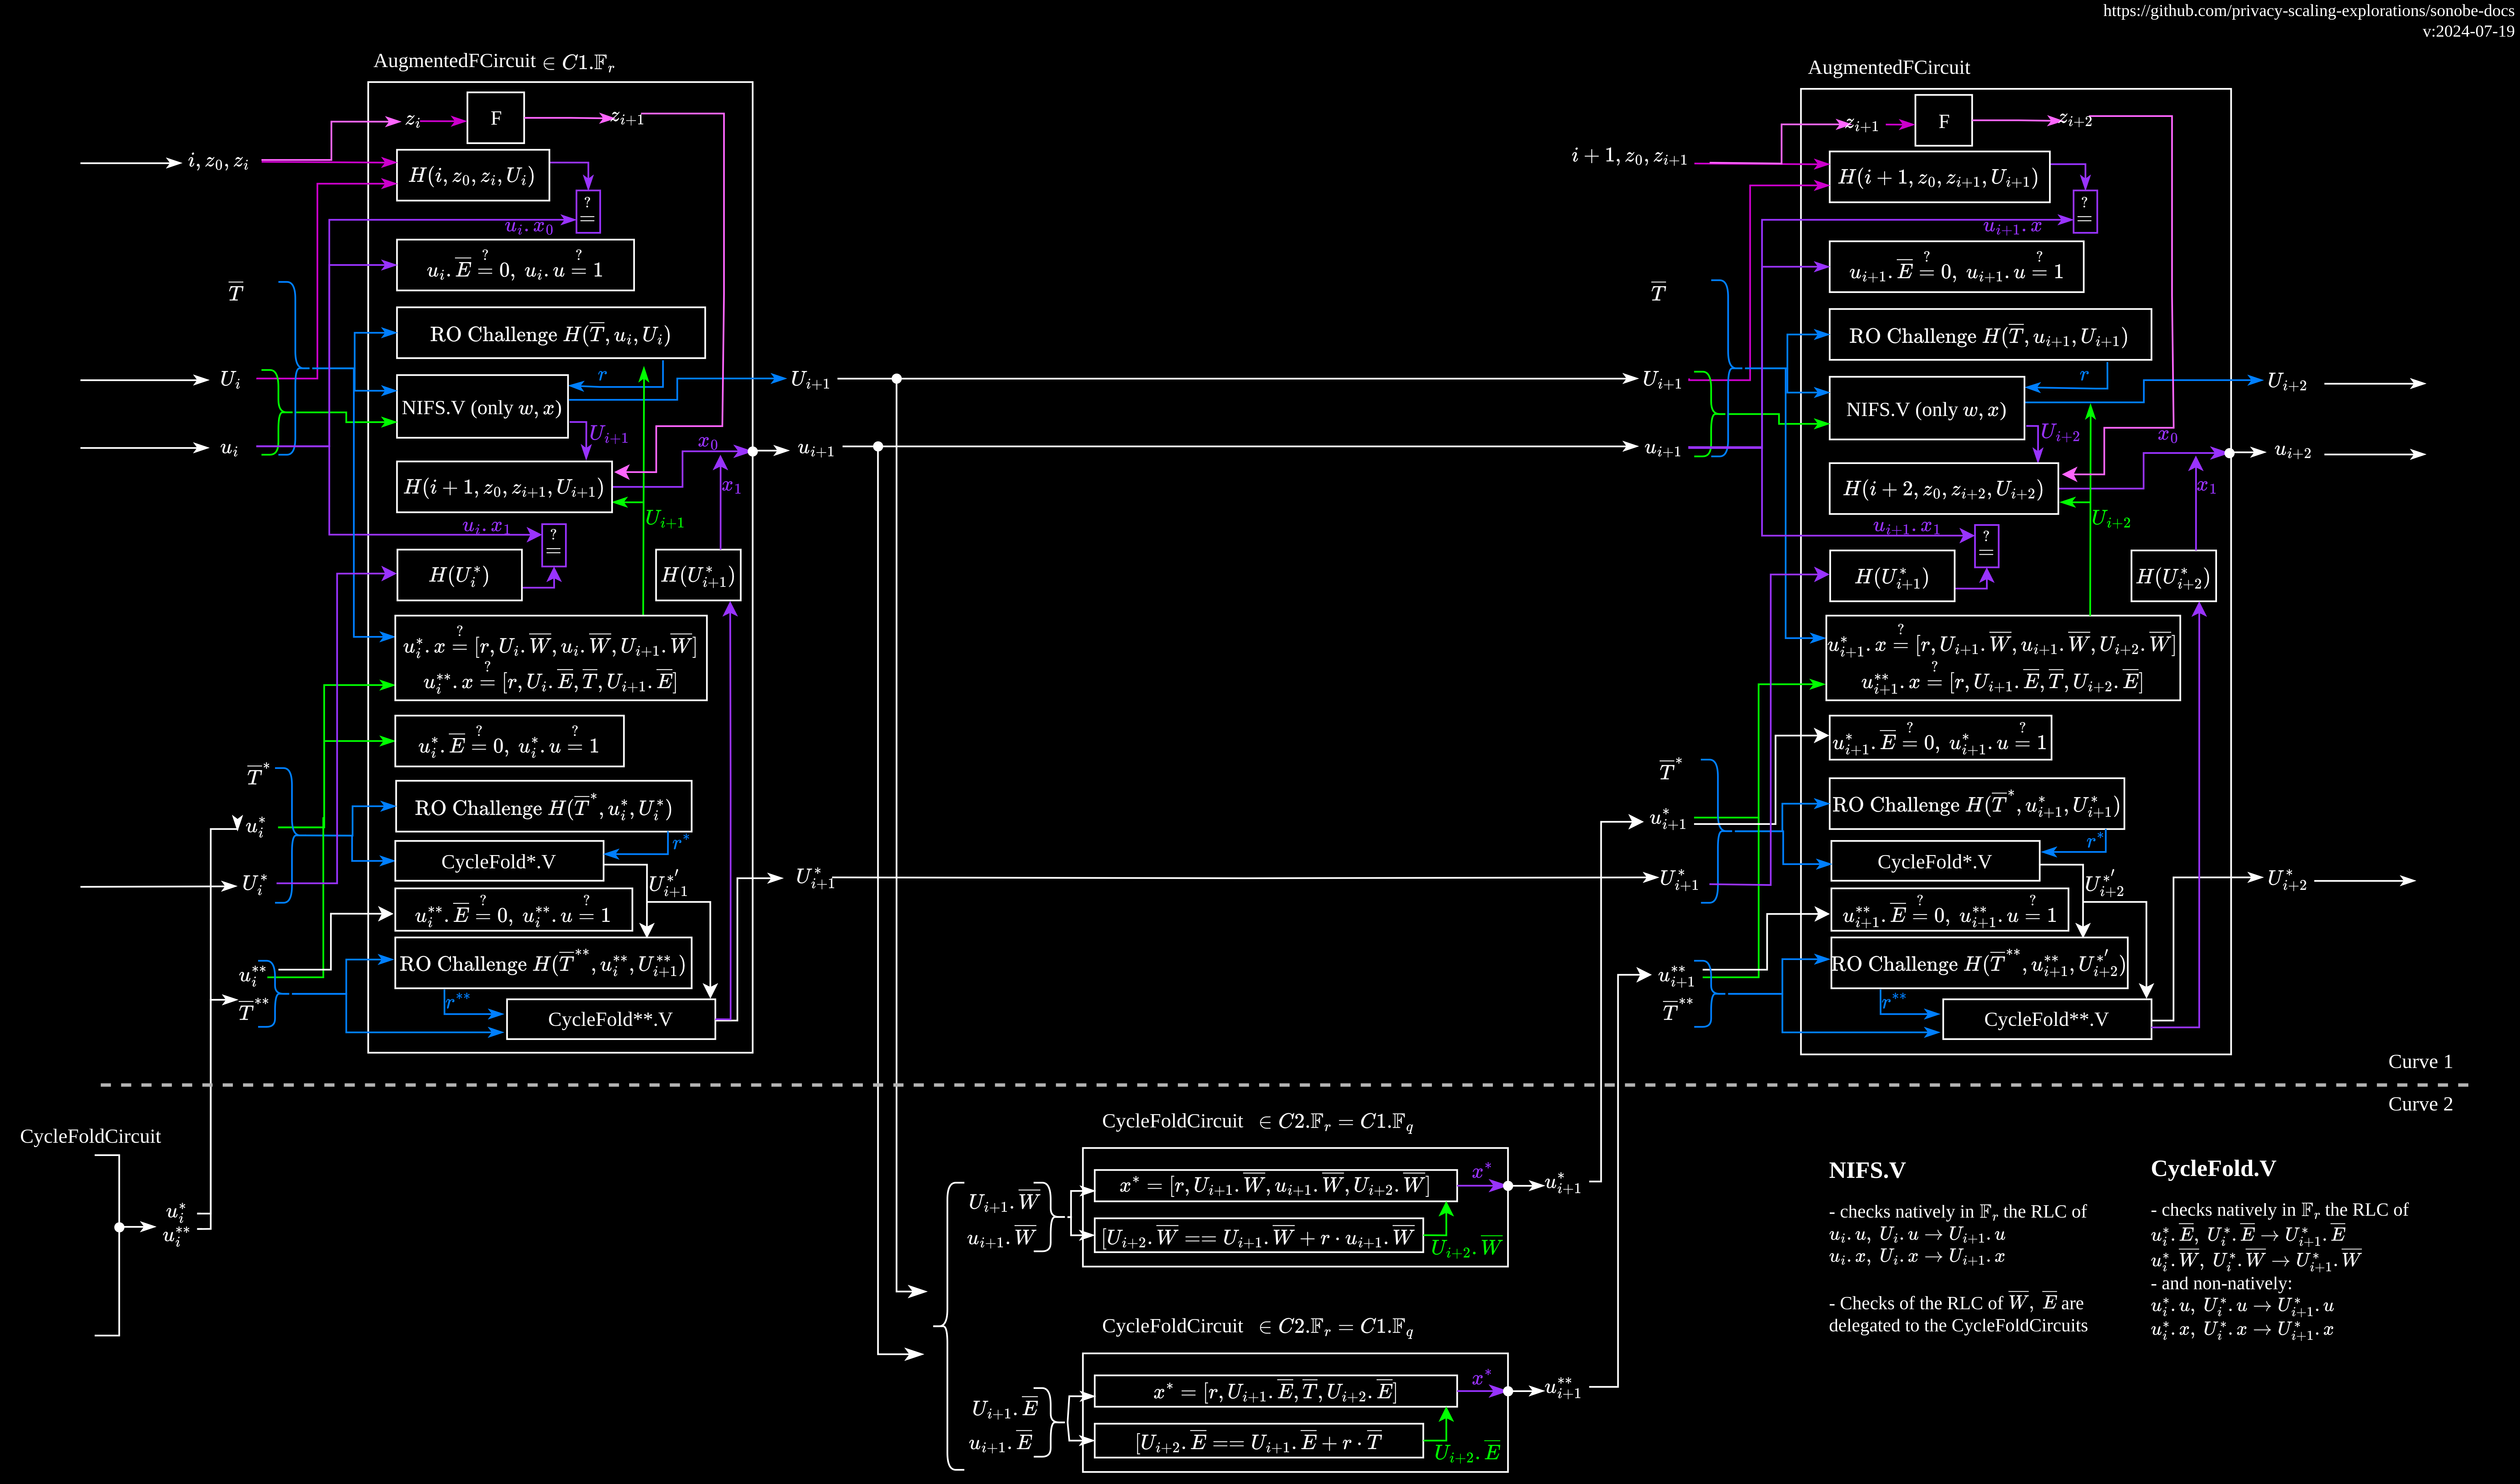
\includegraphics[width=\textwidth]{cyclefold-nova-diagram}
\end{frame}

\begin{frame}{Other Folding Schemes}
  % TODO
  % HyperNova
  % ProtoGalaxy
  % ProtoStar
  % LatticeFold
  % etc
  % mention a bit the different characteristics and folding techniques
\end{frame}

\section{Decider (Final Proof)}

\begin{frame}{Decider}
  \includegraphics[width=\textwidth]{cyclefold-paper-diagram}

  With Prover knowing the respective witnesses for $U_n, u_n, U_{EC,n}$

  \vspace{1cm}

  Issue: IVC proof is not succinct
\end{frame}

\begin{frame}{Decider}
  Original Nova: generate a zkSNARK proof with Spartan for $U_n, u_n, U_{EC, n}$\\
  $\longrightarrow$ 2 Spartan proofs, one on each curve (with CycleFold is 1 Spartan proof)\\
  (not EVM-friendly)

  % draw of the 2 circuits over the curves, and how we generate a Spartan proof for each one

\end{frame}

\begin{frame}{Decider}
  checks (simplified)
  \begin{enumerate}
    \item $(U_{n+1}, W_{n+1})$ satisfy Relaxed R1CS relation of AugmentedFCircuit
    \item verify commitments of $U_{n+1}.\{\overline{E}, \overline{W}\}$ w.r.t. $W_{n+1}.\{E,W\}$
    \item $(U_{EC,n}, W_{EC,n})$ satisfy Relaxed R1CS relation of CycleFoldCircuit
    \item verify commitments of $U_{EC,n}.\{\overline{E}, \overline{W}\}$ w.r.t. $W_{EC,n}.\{E,W\}$
    \item $u_n.E==0,~ u_n.u==1$, ie. $u_n$ is a fresh not-relaxed instance
    \item $u_n.x_0==H(n, z_0, z_n, U_n)$\\
          $u_n.x_1==H(U_{EC,n})$
    \item $NIFS.V(U_n, u_n)==U_{n+1}$
  \end{enumerate}

  % by draw show which are native and not native
  % and that the NIFS.V we do it in Solidity
\end{frame}

\begin{frame}{Decider}
  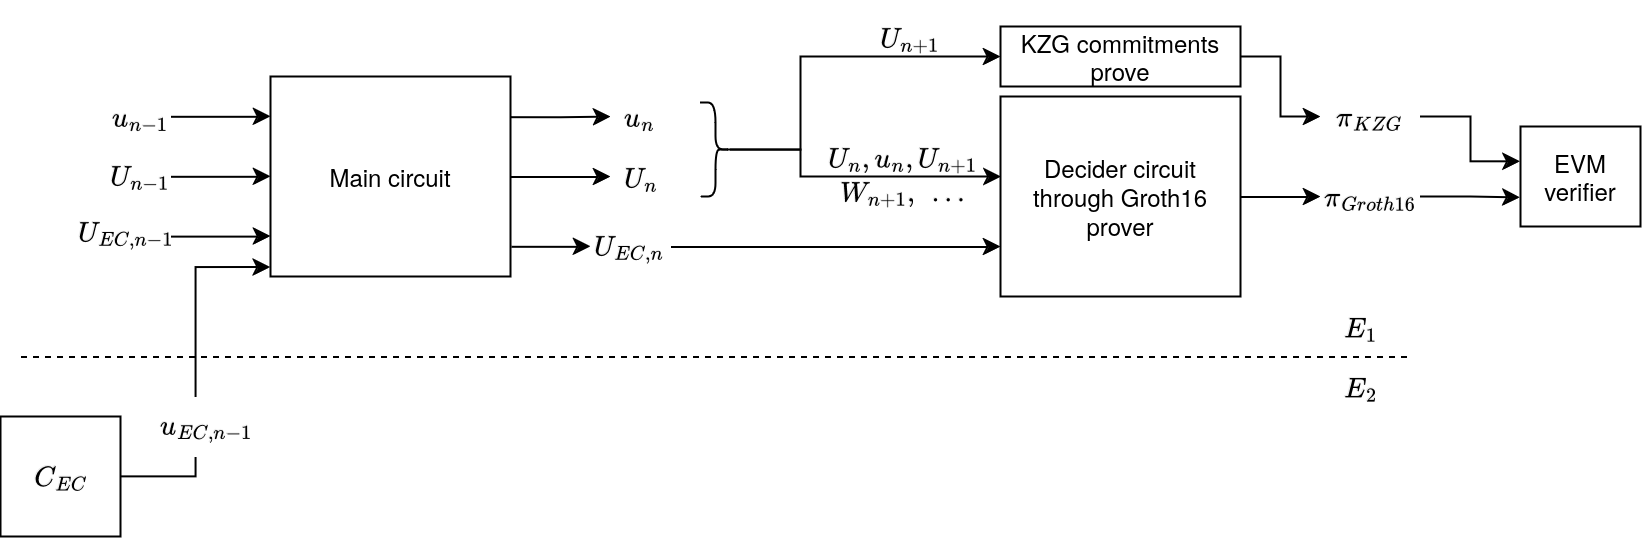
\includegraphics[width=\textwidth]{decider-onchain-flow-diagram}
  % draw of the full flow: from inputting the circuit, to folding to generating the Decider proof to verifying in Ethereum
\end{frame}

\section{Sonobe}
\begin{frame}{Sonobe}
  \footnotesize{
  Experimental folding schemes library implemented jointly by 0xPARC and PSE.

  \vspace{0.3cm}

  Dev flow:
  \begin{enumerate}
    \item Define a circuit to be folded
    \item Set which folding scheme to be used (eg. Nova with CycleFold)
    \item Set a final decider to generate the final proof (eg. Spartan over Pasta curves)
    \item Generate the the decider verifier
  \end{enumerate}
  }

  \vspace{1cm}

  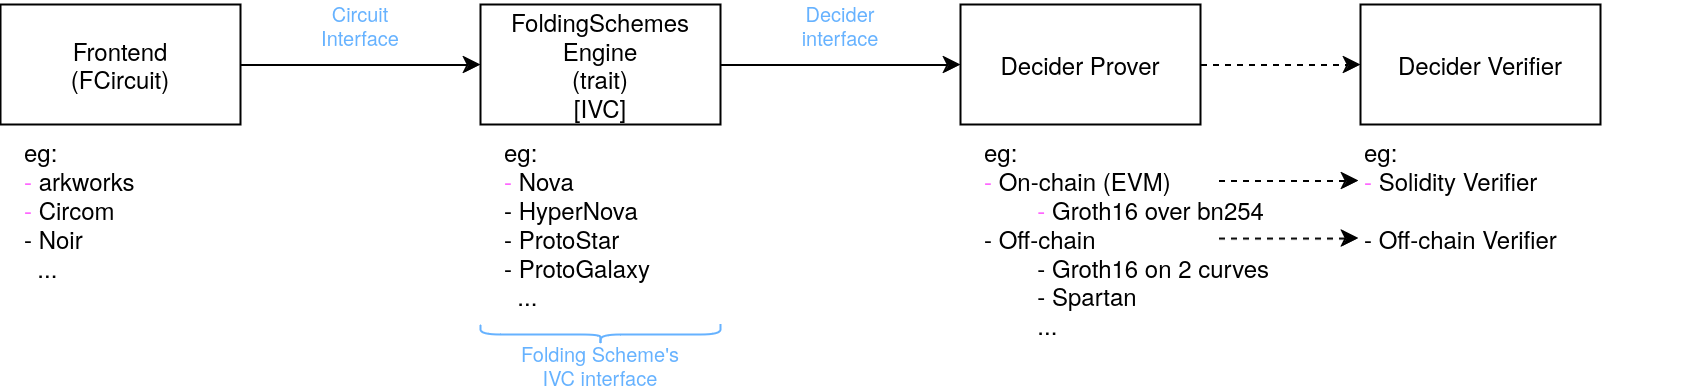
\includegraphics[width=\textwidth]{sonobe-lib-pipeline}
\end{frame}

\begin{frame}{Code example}
  [show code with a live demo]
  \vspace{0.5cm}

  Some numbers (still optimizations pending):
  \begin{itemize}
  \item AugmentedFCircuit: $\sim 80k$ R1CS constraints
  \item DeciderEthCircuit: $\sim 9.6M$ R1CS constraints
  \begin{itemize}
    \item $<3$ minutes in a 32GB RAM 16 core laptop
  \end{itemize}
  \item gas costs (DeciderEthCircuit proof): $\sim 800k$ gas
  \begin{itemize}
    \item mostly from G16, KZG10, public inputs processing
    \item will be reduced by hashing the public inputs
    \item expect to get it down to $< 600k$ gas.
  \end{itemize}
  \end{itemize}

  \vspace{0.3cm}

Recall, this proof is proving that applying $n$ times the function $F$ (the circuit that we're folding) to an initial state $z_0$ results in the state $z_n$.
\\In Srinath Setty words, you can prove practically unbounded computation onchain by 800k gas (and soon $< 600k$).


\end{frame}


\begin{frame}
\frametitle{Wrappup}
\begin{itemize}
  \item \href{https://github.com/privacy-scaling-explorations/sonobe}{https://github.com/privacy-scaling-explorations/sonobe}
  \item \href{https://privacy-scaling-explorations.github.io/sonobe-docs/}{https://privacy-scaling-explorations.github.io/sonobe-docs/}
\end{itemize}

\begin{center}
  \includegraphics[width=4cm]{qr-sonobe-repo-link}
\end{center}

\tiny{
  $$\text{2024-04-22}$$
  $$\text{\href{https://0xparc.org}{0xPARC}~\&~\href{https://pse.dev/}{PSE.}}$$
}
\end{frame}

\end{document}
